\chapter{Разделение секрета}
\selectlanguage{russian}

\section{Пороговые схемы}

Идея \emph{пороговой} $(K, N)$-схемы\index{разделение секрета!пороговое} разделения общего секрета среди $N$ пользователей состоит в следующем. Доверенная сторона хочет распределить некий секрет $K_0$ между $N$ пользователями таким образом, что:
\begin{itemize}
    \item любые $m_1$, $K \leq m_1 \leq N$, легальных пользователей могут получить секрет (или доступ к секрету), если предъявят свои секретные ключи;
    \item любые $m_2$, $m_2 < K$, легальных пользователей не могут получить секрет и не могут определить (вычислить) этот секрет, даже решив трудную в вычислительном смысле задачу.
\end{itemize}

Далее рассмотрены три случая: $(K, N)$-схема Блэкли, $(K, N)$-схема Шамира и простая $(N,N)$-схема.

\subsection[Схема Блекли]{Схема разделения секрета Блекли}\index{схема разделения секрета!Блекли|(}\index{схема разделения секрета!векторная|(}
\selectlanguage{russian}

Схема разделения секрета Блекли (\langen{George Robert Blakley},~\cite{Blackley:1979}), также называемая векторной схемой, основывается на том, что для восстановления всех координат точки в $K$-мерном пространстве, принадлежащей нескольким неколлинеарным гиперплоскостям, необходимо и достаточно знать уравнения $K$ таких плоскостей. То есть в двумерном пространстве нужны две пересекающиеся прямые, в трёхмерном -- три пересекающиеся в нужной точки плоскости и так далее.

\begin{figure}[thb]
	\centering
	\subfloat{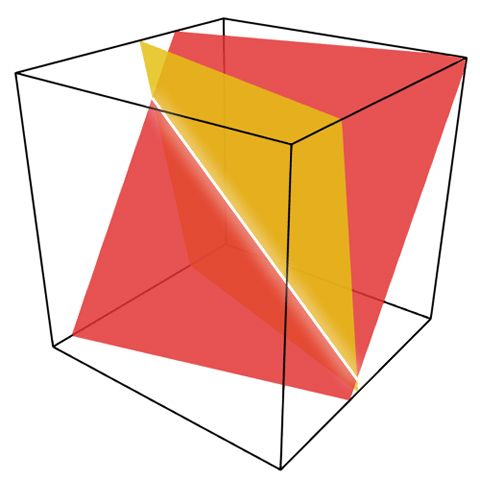
\includegraphics[width=0.45\textwidth]{pic/blakley-2}}
	~~~~
	\subfloat{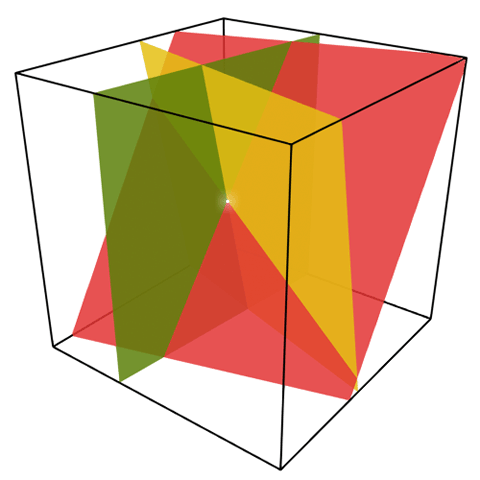
\includegraphics[width=0.45\textwidth]{pic/blakley-3}}
	\caption{Для восстановления координат точки пересечения плоскостей в трёхмерном пространстве необходимо и достаточно знать уравнения трёх таких плоскостей. Данные изображения приведены только для иллюстрации идеи -- в схеме Блекли используется конечное поле, плоскости в котором сложно представить на графике. Рисунок участника English Wikipedia stib, доступно по \href{https://creativecommons.org/licenses/by-sa/3.0/deed.ru}{лицензии CC-BY-SA 3.0}}
\end{figure}

Для разделения секрета $M$ между $N$ сторонами, таким образом, чтобы любые $K$ сторон могли восстановить секрет, доверенный центр выполняет следующие операции:
\begin{itemize}
	\item выбирает несекретное большое простое число $p$ ($p > M$);
	\item выбирает случайную точку, одна из координат которой (например, первая) будет равна разделяемому секрету M: $(x_1 = M, x_2, \dots, x_K)$;
	\item для каждого участника $i$ выбирает $K$ случайных коэффициентов гиперплоскости $C^i_1, C^i_2, \dots, C^i_{K}$ ($\ne 0$), а последний коэффициент $C^i_{K+1}$ вычисляется таким образом, чтобы гиперплоскость проходила через выбранную точку:
		\[ \begin{array}{l}
			C^i_1 x_1 + C^i_2 x_2 + \dots + C^i_K x_K + C^i_{K+1} = 0 \mod p, \\
			C^i_{K+1} = - ( C^i_1 x_1 + C^i_2 x_2 + \dots + C^i_K x_K ) \mod p; \\
		\end{array} \]
	\item раздаёт каждой стороне по следу в виде коэффициентов общего уравнения гиперплоскости $C^i_1, C^i_2, \dots, C^i_{K}, C^i_{K+1}$ и общему модулю $p$.
\end{itemize}

Если стороны могут собраться вместе и получить не менее чем $K$ различных гиперплоскостей, то составив и решив систему уравнений с $K$ неизвестными, они смогут получить все координаты точки $x_1, x_1, \dots, x_k$:

\[ \left\{ \begin{array}{l}
    C^1_1 x_1 + C^1_2 x_2 + \dots + C^1_K x_K + C^1_{K+1} = 0 \mod p, \\
    \dots, \\
    C^K_1 x_1 + C^K_2 x_2 + \dots + C^K_K x_K + C^K_{K+1} = 0 \mod p. \\
\end{array} \right. \]

Если собрано меньшее количество следов (уравнений гиперплоскостей), то их будет недостаточно для решения системы уравнений.

\example
Приведём пример разделения секрета по схеме Блекли в $\GF{11}$. При разделении секрета $M$ используя $(3,N)$ схему Блекли участники получили следы $(4, 8, 2, 6)$, $(2, 6, 8, 3)$, $(6, 8, 4, 1)$. Зная, что следы представляют собой коэффициенты в уравнении плоскости общего вида, а исходный секрет -- первую координату точки пересечения плоскостей, составляем систему уравнений для нахождения координаты этой точки:

\[ \left\{\begin{align}
   \left( 4\cdot x_1 + 8\cdot x_2 + 2\cdot x_3 + 6 \right) &= 0 &\mod 11  \\
   \left( 2\cdot x_1 + 6\cdot x_2 + 8\cdot x_3 + 3 \right) &= 0 &\mod 11  \\
   \left( 6\cdot x_1 + 8\cdot x_2 + 4\cdot x_3 + 1 \right) &= 0 &\mod 11  \\
\end{align} \right. \]

Решением данной системы будет являться точка (6, 4, 2), а её первая координата -- разделяемый секрет.
\exampleend

\index{схема разделения секрета!векторная|)}\index{схема разделения секрета!Блекли|)}


\subsection[Схема Шамира]{Схема разделения секрета Шамира}\index{схема разделения секрета!Шамира|(}\index{схема разделения секрета!интерполяционных полиномов Лагранжа|(}
\selectlanguage{russian}

Схема разделения секрета Шамира (\langen{Adi Shamir},~\cite{Shamir:1979}), также называемая схемой интерполяционных полиномов Лагранжа, основывается на том, что для восстановления всех коэффициентов полинома $P(x) = a_{K-1}x^{K-1} + \dots + a_1 x + a_0$ степени $K-1$ требуется $K$ координат различных точек, принадлежащих кривой $y=P(x)$. Все операции проводятся в конечном поле $GF(p)$.

\begin{figure}[thb]
	\centering
	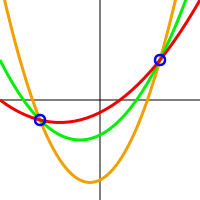
\includegraphics[width=0.5\textwidth]{pic/shamir}
  \caption{Через две точки можно провести неограниченное число графиков, заданных полиномами степени 2. Чтобы выбрать из них единственный -- нужна третья точка. Данные графики приведены только для иллюстрации идеи -- в схеме Шамира используется конечное поле, полиномы над которым сложно представить на графике}
  \label{fig:shamir}
\end{figure}

Для разделения секрета $M$ между $N$ сторонами таким образом, чтобы любые $K$ сторон могли восстановить секрет, доверенный центр выполняет следующие операции:
\begin{itemize}
	\item выбирает несекретное большое простое число $p$ ($p > M$);
	\item в качестве свободного члена секретного многочлена полагает разделяемый секрет $a_0 = M$;
	\item выбирает остальные секретные коэффициенты многочлена $a_1, \dots, a_{k-1}$, меньшие $p$;
	\item выбирает $N$ различных $x$, таких что $0 < x_i < p$;
	\item для каждого выбранного $x_i$ вычисляет соответствующий $y_i$, подставляя значения в формулу многочлена
		\[ y_i = P( x_i ) = a_{K-1}x_i^{K-1} + \dots + a_1 x_i + a_0 \mod p ;\]
	\item раздаёт каждой стороне по следу вида $(x_i, y_i)$ и общему модулю $p$.
\end{itemize}

Если стороны могут собраться вместе и получить не менее чем $K$ различных следов, то, составив и решив систему уравнений с $K$ неизвестными, они смогут получить все коэффициенты $a_0, a_1, \dots, a_{k-1}$ секретного многочлена:

\[ \left\{ \begin{array}{l}
    y_1 = a_{K-1}x_1^{K-1} + \dots + a_1 x_1 + a_0 \mod p, \\
    \dots, \\
    y_k = a_{K-1}x_k^{K-1} + \dots + a_1 x_k + a_0 \mod p. \\
\end{array} \right. \]

Если собрано меньшее количество следов, то их будет недостаточно для решения системы уравнений.

Существует также способ вычисления коэффициентов многочлена, основанный на методе интерполяционных полиномов Лагранжа (откуда и берётся второе название метода разделения секрета). Идея способа состоит в вычислении набора специальных полиномов $l_i \left( x \right)$, которые принимают значение $1$ в точке $x_i$, а во всех остальных точках-следах их значение равно нулю:

\[ \begin{cases}
	l_i \left( x_j \right) = 1, x_j = x_i, \\
	l_i \left( x_j \right) = 0, x_j \ne x_i. \\
\end{cases} \]

Далее эти многочлены умножаются на значения $y_i$ и в сумме дают исходный многочлен:
\[\begin{array}{llll}
  l_i \left( x \right) &=& \prod\limits_{j \ne i} {\frac{{x - x_j }}{{x_i  - x_j }}} &\mod p, \\
  F\left( x \right) &=& \sum\limits_i {l_i \left( x \right)y_i } &\mod p. \\
\end{array}\]

Строго говоря, для восстановления самого секрета, которым является свободный член многочлена, не обязательно восстанавливать весь многочлен, а можно использовать упрощённую формулу для восстановления только свободного члена $a_0 = M$:
    \[ M = \sum\limits_{i=0}^{k-1} y_i \prod\limits_{j=0, j \neq i}^{k-1} \frac{x_j}{x_j - x_i}. \]

\example
Приведём схему Шамира в поле $\GF{p}$. Для разделения секрета $M$ в $(3,n)$-пороговой схеме используется многочлен степени $3-1=2$.
    \[ f(x) = a x^2 + b x + M \mod p, \]
где $p$ -- простое\index{число!простое} число. Пусть $p=23$. Восстановим секрет $M$ по \emph{теням}
    \[ (1,14), (4,21), (15,6). \]

Последовательно вычисляем
\[\begin{array}{l}
	M = \sum\limits_{i=0}^{k-1} y_i \prod\limits_{j=0, j \neq i}^{k-1} \frac{x_j}{x_j - x_i} \mod p = \\
	= 14 \cdot \frac{4}{4-1} \cdot \frac{15}{15-1} + 21 \cdot \frac{1}{1-4} \cdot \frac{15}{15-4} + 6 \cdot \frac{1}{1-15} \cdot \frac{4}{4-15} \mod 23 = \\
	= 14 \cdot \frac{4}{3} \cdot \frac{15}{14} + 21 \cdot \frac{1}{-3} \cdot \frac{15}{11} + 6 \cdot \frac{1}{-14} \cdot \frac{4}{-11} \mod 23 = \\
	= 20 - 7 \cdot 15 \cdot 11^{-1} + 12 \cdot 7^{-1} \cdot 11^{-1} \mod 23 = \\
	= 13 \mod 23. \\
\end{array}\]

\exampleend

\index{схема разделения секрета!интерполяционных полиномов Лагранжа|)}\index{схема разделения секрета!Шамира|)}


\subsection[$(N, N)$-схема]{$(N, N)$-схема разделения секрета}
\selectlanguage{russian}

Рассмотрим пороговую схему распределения одного секрета между двумя легальными пользователями. Она обозначается как $(2,2)$-схема -- это означает, что оба и только оба пользователя могут получить секрет. Предположим, что секрет $K_{0}$ -- это двоичная последовательность длины $M$, $K_{0} \in \Z_{M}$.

Разделение секрета $K_{0}$ состоит в следующем.
\begin{itemize}
    \item Первый пользователь в качестве секрета получает случайную двоичную последовательность $A_{1}$ длины $M$.
    \item Второй пользователь в качестве секрета получает случайную двоичную последовательность $A_{2} =K_{0} \oplus A_{1}$ длины $M$.
    \item Для получения секрета $K_{0}$ оба пользователя должны сложить по модулю 2 свои секретные ключи (последовательности)  $K_{0} = A_{2} \oplus A_{1}$.
\end{itemize}

Теперь рассмотрим пороговую $(N,N)$-схему.

Имеется общий секрет $K_{0} \in \Z_{M}$ и $N$ легальных пользователей, которые могут получить секрет только в случае, если одновременно предъявят свои секретные ключи. Распределение секрета $K_{0}$ происходит следующим образом:

\begin{itemize}
    \item Первый пользователь в качестве секрета получает случайную двоичную последовательность $A_{1} \in \Z_{M}$.
    \item Второй пользователь в качестве секрета получает случайную двоичную последовательность $A_{2}\in \Z_{M}$ и т.~д.
    \item $(N-1)$-й пользователь в качестве секрета получает случайную двоичную последовательность $A_{N-1}\in \Z_{M}$.
    \item $N$-й пользователь в качестве секрета получает двоичную последовательность
        \[ K_0 \oplus A_1 \oplus A_2 \oplus \dots \oplus A_{N-1}. \]
    \item Для получения секрета $K_0$ все пользователи должны сложить по модулю 2 свои последовательности:
        \[ A_1 \oplus A_2 \oplus \dots \oplus A_{N-1} \oplus (K_0 \oplus A_1 \oplus A_2 \dots \oplus A_{N-1}) = K_0. \]
\end{itemize}

Предположим, что собравшихся вместе пользователей меньше общего числа $N$, например, всего $N-1$ первых пользователей. Тогда суммирование $N-1$ последовательностей не определяет секрета, а перебор невозможен, так как данная схема разделения секрета аналогична криптосистеме Вернама и обладает совершенной криптостойкостью.


\section{Распределение секрета по коалициям}

\subsection{Схема для нескольких коалиций}

Предположим, что имеется $N$ легальных пользователей
    \[ \{ U_1, U_2, \dots, U_N \}, \]
которым нужно сообщить (открыть, получить доступ к) общий секрет $K$.

Секрет может быть доступен только определённым коалициям\index{распределение секрета!по коалициям}, например:
\[ \begin{array}{l}
    C_1 = \{ U_1, U_2 \}, \\
    C_2 = \{ U_1, U_3, U_4 \}, \\
    C_3 = \{ U_2, U_3 \}, \\
    \dots
\end{array} \]
При этом ни одна из коалиций $C_i, ~ i = 1, 2, \dots$ не должна быть подмножеством другой коалиции.


\example
Имеется 4 участника:
    \[ \{ U_1, U_2, U_3, U_4 \}, \]
которые образуют 3 коалиции:
\[ \begin{array}{l}
    C_1 = \{ U_1, U_2 \}, \\
    C_2 = \{ U_1, U_3 \}, \\
    C_3 = \{ U_2, U_3, U_4 \}. \\
\end{array} \]
Распределение частичных секретов между ними представлено в виде таблицы~\ref{tab:secret-share-coalition-1}, в которой введены следующие обозначения: $a_1, b_1, c_2, c_3$ -- случайные числа из кольца $\Z_M$. В строках таблицы содержатся частичные секреты каждого из пользователей, в столбцах таблицы показаны частичные секреты, соответствующие каждой из коалиций.

\begin{table}[!ht]
    \centering
    \caption{Распределение секрета по определённым коалициям\label{tab:secret-share-coalition-1}}
    \begin{tabular}{|c||c|c|c|}
        \hline
              & $C_1 = \{ U_1, U_2 \}$ & $C_2 = \{U_1, U_3 \}$ & $C_3 = \{ U_2, U_3, U_4 \}$ \\
        \hline \hline
        $U_1$ & $a_1$     & $b_1$     & -- \\
        $U_2$ & $K - a_1$ & --        & $c_2$ \\
        $U_3$ & --        & $K - b_1$ & $c_3$  \\
        $U_4$ & --        & --        & $K - c_2 - c_3$ \\
        \hline
    \end{tabular}
\end{table}

Как видно из приведённых данных, суммирование по модулю $M$ чисел, приведённых в каждом из столбцов таблицы, открывает секрет $K$.
\exampleend


\example

%\section{Схема разделения секрета на монотонных булевых функциях}
%\example
В системе распределения секрета доверенный
%с использованием монотонных булевых функций
центр использует кольцо $\Z_m$ целых чисел по модулю $m$. Требуется разделить секрет $K$ между $5$ пользователями:
    \[ \{ U_1, U_2, U_3, U_4, U_5 \} \]
так, чтобы восстановить секрет могли только коалиции:
\[ \begin{array}{lll}
    C_1 = \{ U_1, U_2 \},      & & C_2 = \{ U_1, U_3 \}, \\
    C_3 = \{ U_2, U_3, U_4 \}, & & C_4 = \{ U_2, U_3, U_5 \}, \\
    C_5 = \{ U_3, U_4, U_5 \}, & & C_6 = \{ U_1, U_2, U_3 \}. \\
\end{array} \]

Заданное множество коалиций с доступом не является минимальным, так как одни коалиции входят в другие:
    \[ C_1 \subset C_6, ~ C_2 \subset C_6. \]
Исключая $C_6$, получим минимальное множество коалиций с доступом к секрету -- ни одна из оставшихся коалиций не входит в другую $C_i \nsubseteq C_j$ для $i \neq j$. Пользователям выдаются тени по минимальному множеству коалиций с доступом. В строках таблицы~\ref{tab:secret-share-coalition-2} содержатся частичные секреты каждого из пользователей, в столбцах таблицы показаны частичные секреты, соответствующие каждой из коалиций.

\begin{table}[!ht]
    \centering
    \caption{Распределение секрета по определённым коалициям\label{tab:secret-share-coalition-2}}
    \begin{tabular}{|c||c|c|c|c|c|}
        \hline
              & $C_1$     & $C_2$     & $C_3$           & $C_4$           & $C_5$  \\
        \hline \hline
        $U_1$ & $a_1$     & $b_1$     & --              & --              & -- \\
        $U_2$ & $K - a_1$ & --        & $c_2$           & $d_2$           & --\\
        $U_3$ & --        & $K - b_1$ & $c_3$           & $d_3$           & $e_3$ \\
        $U_4$ & --        & --        & $K - c_2 - c_3$ & --              & $e_4$ \\
        $U_5$ & --        & --        & --              & $K - d_2 - d_3$ & $K - e_3 - e_4$ \\
        \hline
    \end{tabular}
\end{table}

Тени выбираются случайно из кольца $\mathbb{\Z}_m$. В результате у пользователей будут тени. 
\exampleend

\subsection{Схема Брикелла для нескольких коалиций}\index{схема распределение секрета!Бриккела|(}
\selectlanguage{russian}

Рассмотрим схему Брикелла (\langen{Ernest Francis Brickell},~\cite{Brickell:1990}) распределения секрета по коалициям.

По-прежнему
    \[ \{ U_1, U_2, \dots, U_N \} \]
-- легальные пользователи. Пусть $\Z_p$ -- кольцо целых чисел по модулю $p$. Рассмотрим векторы
    \[ \mathcal{U} = \left\{ (u_1, u_2, \dots, u_d) \right\}, ~~ u_i \in \Z_p \]
длины $d$. Каждому пользователю $U_i, ~ i = 1, \dots, N$ ставится в соответствие вектор
    \[ \varphi(U_i) \in \mathcal{U}, ~~ i = 1, \dots, N. \]

Тогда каждой из коалиций, например
    \[ C_1 = \{ U_1, U_2, U_3 \}, \]
соответствует набор векторов
    \[ \varphi(U_1), \varphi(U_2), \varphi(U_3). \]
Эти векторы должны быть выбраны так, чтобы их линейная оболочка \emph{содержала} вектор
    \[ (1, 0, 0, \dots, 0) \]
длины $d$. Линейная оболочка любого набора векторов, не образующих коалицию, \emph{не должна} содержать вектор $(1, 0, 0, \dots, 0)$ длины $d$.

Пусть $K_0 \in \Z_p$ -- общий секрет. Распределение секрета производится следующим образом. Сначала вычисляется вектор $(K_0, K_1, \dots, K_{d-1})$, где первая координата -- это общий секрет, а остальные координаты выбираются из $\Z_p$ случайно. Затем вычисляются скалярные произведения:
\[\begin{array}{l}
	\left( \left( K_0, K_1, \dots, K_{d-1} \right), ~ \varphi(U_1) \right) ~=~ a_1, \\
	\left( \left( K_0, K_1, \dots, K_{d-1} \right), ~ \varphi(U_2) \right) ~=~ a_2, \\
	\dots \\
	\left( \left( K_0, K_1, \dots, K_{d-1} \right), ~ \varphi(U_N) \right) ~=~ a_N. \\
\end{array}\]

Пользователям $U_i, ~ i = 1, 2, \dots, N$ выдаются их частичные секреты:
    \[ U_i \colon \left\{ \varphi(U_i), a_i \right\}. \]

Пусть коалиция $C$ -- допустимая, например:
    \[ C = C_1 = \{ U_1, U_2, U_3 \}. \]

Тогда члены коалиции совместно находят такие коэффициенты $\lambda_1, \lambda_2, \lambda_3$, что
    \[ \lambda_1\varphi(U_1)+\lambda_2\varphi(U_2)+\lambda_3\varphi(U_3) ~=~ (1,0, \dots, 0). \]

После этого вычисляется выражение
\[\begin{array}{l}
    \lambda_1 a_1 + \lambda_2 a_2 + \lambda_3 a_3 = \\
    = \left( \left( K_0, K_1, \dots, K_{d-1} \right), ~ \lambda_1 \varphi(U_1) + \lambda_2 \varphi(U_2) + \lambda_3 \varphi(U_3) \right) = \\
    = \left( \left( K_0, K_1, \dots, K_{d-1} \right), ~ \left( 1, 0, \dots, 0 \right) \right) =  K_0, \\
\end{array}\]
которое и является общим секретом.

%\section{Схема разделения секрета в векторном пространстве Бриккела}
%
%В схеме Бриккела для $n$ пользователей $\{ U_1, U_2, \ldots, U_n \}$ Центр выбирает $k$-мерные векторы $\varphi(U_i)$ над полем $\mathbb{\Z}_p$ так, чтобы их линейная нетривиальная комбинация над полем $\mathbb{\Z}_p$ могла равняться единичному вектору
%    \[ (1,0,0, \ldots, 0) = \sum\limits_{i=1}^{n} c_i \ \varphi(U_i), ~ c_i \in  \mathbb{\Z}_p. \]
%Центр пользователю $i$ присваивает \emph{открытый, публично доступный} вектор $\varphi(U_i)$.
%
%Для разделения секрета $K$ Центр выбирает случайные числа $a_2, a_3, \ldots, a_n$, составляет вектор $\bar{a} = (K, a_2, a_3, \ldots, a_n)$ и выдаёт каждому пользователю \emph{секретную} тень $s_i = \bar{a} \cdot \varphi(U_i)$.
%
%Восстановление секрета производится
%    \[ K = \bar{a} \cdot (1,0,\ldots,0) = \bar{a} \cdot \sum\limits_{i=1}^{n} c_i \varphi(U_i) = \sum\limits_{i=1}^{n} c_i s_i, \]
%так как из открытых векторов $\varphi(U_i)$ пользователи могут найти $c_i$.
%
%Восстановить секрет могут только те коалиции пользователей, для которых нетривиальная комбинация векторов $\varphi(U_i)$ даёт единичный вектор.

\example
Для сети из $n = 4$ участников
    \[ \{ U_1, U_2, U_3, U_4 \} \]
выбраны следующие векторы длины $k = 3$ над полем $\Z_{23}$:
\[ \begin{array}{l}
    \varphi(U_1) = (0,2,0), \\
    \varphi(U_2) = (2,0,7), \\
    \varphi(U_3) = (0,5,7), \\
    \varphi(U_4) = (0,2,9). \\
\end{array} \]
Найдём все коалиции, которые могут раскрыть секрет.

Запишем
    \[ (1,0,0) = c_1 (0,2,0) + c_2 (2,0,7) + c_3 (0,5,7) + c_4 (0,2,9). \]
Ясно, что $c_2 \neq 0$ и коалициями пользователей, которые дают единичный вектор и, следовательно, могут восстановить секрет, являются:
\[ \begin{array}{l}
    C_1 = \{ U_1, U_2, U_3 \}, \\
    C_2 = \{ U_1, U_2, U_4 \}, \\
    C_3 = \{ U_2, U_3, U_4 \}. \\
\end{array} \]

Пусть доверенный центр для секрета $K = 4$ выбрал вектор $\bar{a} = (4, 2, 9)$. Тогда участники получают тени:
    \[ s_1 = (4,2,9) \cdot (0,2,0) = 4 \mod 23, \]
    \[ s_2 = (4,2,9) \cdot (2,0,7) = 2 \mod 23, \]
    \[ s_3 = (4,2,9) \cdot (0,5,7) = 4 \mod 23, \]
    \[ s_4 = (4,2,9) \cdot (0,2,9) = 16 \mod 23. \]

Возьмём коалицию $C_1 = \{ U_1, U_2, U_3 \}$ и вычислим коэффициенты $c_i$:
    \[ (1,0,0) = c_1 (0,2,0) + c_2 (2,0,7) + c_3 (0,5,7), \]
\[ \begin{array}{l}
    c_1 = 7 \mod 23, \\
    c_2 = 12 \mod 23, \\
    c_3 = 11 \mod 23. \\
\end{array} \]

Найдём секрет:
    \[ K = 7 \cdot 4 + 12 \cdot 2 + 11 \cdot 4 = 4 \mod 23.\]
\exampleend

\index{схема распределение секрета!Бриккела|)}

